\lhead{\emph{\leftmark}}  

\chapter{Detection Mechanisms for UML/Umple Constructs}
\label{chap:detections}

In this chapter we will present the different mechanisms to detect UML/Umple attributes, associations and state machines from source code written in an object-oriented programming language. We started to build our detection rules based on the following::

\begin{enumerate}

\item Documented implementations of attributes, associations and state machines in high level programming languages mentioned in the literature. In particular, we have considered research that discusses how to generate code from this modeling concepts (Forward engineering).

\item Documented techniques in the literature for discovering  modeling constructs in object-oriented source code (Reverse Engineering).

\item Our own analysis of open source systems written in object-oriented programming languages.

\end{enumerate}

To present the set of transformation rules we developed from the above, we will employ a semi-formal notation. The rules define the transformation from input to output. It must be pointed out that these transformations rules can be described using a metamodel-based language or grammar-based language. Both types of descriptions allow us to specify mappings between source and target models in the form of conditions (patterns) and conversions (replacements) executed from input to output when those conditions hold. As the intent of our work is to transform object-oriented  language programs into umple programs, we will employ a metamodel-based approach to better express the input/output relationships. The metamodel-based language will be enhanced with OCL \cite{WarmerOCL2003} expressions. 
% create table in chapter 5, showing m2t and m2m requirements in terms of Model source code
% M2M: UmpleModel, JavaModel
% M2T: JavaModel, UmpleCode
% T2T: Java code, Umple Code

\section{A Notation for Transformation Rules}
\label{sec:2ModelTransformation}

Transformation rules presented in this chapter will contain the following information:

\begin{enumerate}

\item A name for each transformation rule used for reference purposes.

\item The source language reference

\item Constants used in the generation of the target

\item Helper methods used in the extraction of information from target or input models.

\item A set of named source language model elements from the source language metamodel that we call B.

\item A set of named target language model elements from the target language metamodel that we call U.

\item The source language conditions: invariants that state the conditions that must hold in the source model for this transformation to be applied.

\item The target language conditions: invariants that state the conditions that must hold in the target model for this transformation to be applied.

\end{enumerate}

% It would be better in this template if the keyword 'conditions' and 'mappings' would be in blue, just like 'in' and 'out'
% MG Fixed

Listing \ref{lst:templateTransform} presents a template definition for the transformations rules.

\begin{lstlisting}[style=mine,caption=Template definition for Transformation rules,label=lst:templateTransform]
Transformation Name  (InputModel, OutputModel){
 order n
 params
 	...
 in
   sourceElement: ...
 out
   targetElement: ...
 in conditions
    ...
 out conditions
 	...
 mappings
    sourceElement.propertyA -> targetElement.propertyA;
    sourceElement.propertyB -> targetElement.propertyB;
}
\end{lstlisting}

The various parts of a transformation rule have their own  specific notation:

\begin{itemize}

\item Line 1. Every transformation possess a name. The source and target languages are referenced by stating both language names after the transformation name.

\item Line 2. The order of application of the rule is determined by the integer number following the keyword \textit{order}. Rules with lower order numbers are executed first. Order of application of the rules doesn't matter when two or more rules possess the same order number. 

\item Line 3. Local and global variables to be used in the transformation rule are specified following the keyword \textit{params}.

\item Lines 5 and 7. The source model and target elements are written as variable declarations following the keywords \textit{in} and \textit{out} respectively.

\item Lines 9 and 11. The conditions that must hold on the source and target model elements are specified following the keywords \textit{in conditions} and \textit{out conditions} respectively. The mappings are performed only if both the in and out conditions are true. Conditions can be specified using OCL syntax. 

\item Line 13. The mapping rules come after the keyword \textit{mappings}. The symbol -\textgreater  is used as an infix operator with two operands. The symbol specifies a transformation of the left hand side operand to the right side operand (rules are unidirectional).
\end{itemize}

We will now introduce the transformation rules for each of the transformation steps presented in Chapter \ref{chap:core}.
The set of rules for each transformation case constitutes a transformation case definition. Rules in the set are to be executed in sequence.

\section{Transformation Rules for the Initial Transformation Step}

Transformations rules for this step are straightforward and aim at transforming the package declaration, namespace declarations, import declaration and the generalization notation into the corresponding Umple notation. 

The mapping rule in Listing \ref{lst:4.1.1} specifies the transformation of a Class into an Umple class using the language defined in the previous section. A type declaration in the base language model represents an object-oriented type (i.e., a class, interface, struct, etc). The only required condition in the rule shown in Listing \ref{lst:4.1.1} (Line 7) is that the \textit{typeDeclaration} must declare a class and not an interface or abstract class. A very similar rule is then required for the transformation of a \textit{typeDeclaration} into an Umple Interface. The relationship between the source model, the target model and the mapping rule (in blue background) are illustrated in Figure \ref{fig:4.1.1}.
Transformation rules defined in a general but formal language can then be adapted to specific languages such as Java or C++. For instance, the name of a typeDeclaration if the input language is Java can be extracted using the \textit{getName().getFullyQualifiedName()} call sequence. Actual implementation of the mapping rules will be presented in Chapter \ref{chap:tool}. For our first example, we show the BNF grammar for a type declaration in Java and an Umple class declaration in Listings \ref{lst:javaGrammar1} and \ref{lst:umpleGrammar2} respectively. It must be pointed out that the transformation rule can be understood either by looking at the metamodel or the grammar of input/output models. 

% The following Listing is totally mixed up with the subsequent figure in the tool, but when I export a pdf it looks OK. Very strange.
% MG. Strange, I see the same problem. PDF will be fine however.

% Also, you are using tabs, which Latex doesn't process properly in listings. You need to use two spaces instead of tabs. I have made this change in this case, but make the change elsewhere and watch out in other code.
% Fixed MG.

% Readers will be confused as to the detailed sublanguages (e.g. the reference to isInterface(), ::TypeDeclariation, .name and so on. How are you going to define these? I know you say this is 'informal' (actually I changed it to 'semiformal' which is the correct term), but nonetheless it should be understandable. Are you referring to JDT contstructs? If so then there is the problem that you haven't introduced JDT yet. Perhaps the solution is to put much of Chapter 5 before this (discussing how you tried ATL, TXL and then briefly xDT), then have this chapter, which can now refer to JDT, and finally discuss the implification in another separate chapter. There would end up being one more chapter than there is now.
% But there may be another way to make this all make sense, such as defining the semi-formal language in a simple way here.
% MG Fixed by using a more abstract way of presenting the language. 

\begin{lstlisting}[style=mine,caption=Grammar for Java Types,label=lst:javaGrammar1]
TypeDeclaration:
                ClassDeclaration
                InterfaceDeclaration
 ClassDeclaration:
      [ Javadoc ] { Modifier } class Name
                        [ extends Type]
                        [ implements Type { , Type } ]
                        { { ClassBodyDeclaration | ; } }
 InterfaceDeclaration:
      [ Javadoc ] { Modifier } interface Identifier
                        [ extends Type { , Type } ]
                        { { InterfaceBodyDeclaration | ; } }
\end{lstlisting}

\begin{lstlisting}[style=mine,caption=Grammar for Umple Classes,label=lst:umpleGrammar2]
 umpleClass : class Name { [[classContent]]* }
\end{lstlisting}

\begin{lstlisting}[style=mine,caption=Rule BaseTypeToUmpleClass,label=lst:4.1.1]
Transformation BaseTypeToUmpleClass (BaseLanguageMetamodel, UmpleMetamodel){ 
 in
   typeDeclaration : BaseLanguageModel::TypeDeclaration;
 out
   UmpleClass: UmpleMetamodel::UmpleClass;
 in conditions
   oclIsTypeOf(ClassDeclaration);   
 mappings
   typeDeclaration.name -> UmpleClass.name;
}
\end{lstlisting}

\begin{figure}[h]
\centering
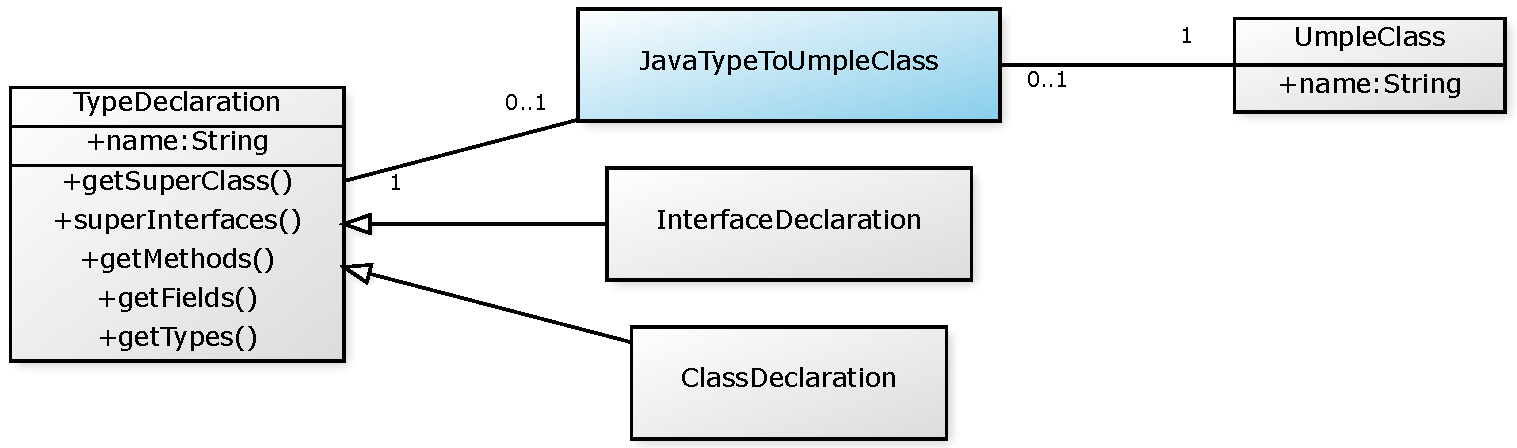
\includegraphics[width=0.99\textwidth]{Figures/ch4InitialMapping.pdf}
\caption{Input-Output relationships for rule BaseTypeToUmpleClass}
\label{fig:4.1.1}
\end{figure}

Similarly, rule  \textit{ImportToUmpleDepend} in Listing \ref{lst:4.1.2} specifies the transformation of a import declaration into a depend declaration. Import directives in object-oriented languages are used to incorporate information from a type library. 

\begin{lstlisting}[style=mine,caption=Rule JavaImportToUmpleDepend,label=lst:4.1.2]
Transformation ImportToUmpleDepend (BaseLanguageMetamodel, UmpleMetamodel){ 
 in
   importDeclaration : BaseLanguageModel::ImportDeclaration;
 out
   depend: UmpleMetamodel::Depend;
 in-out conditions
   UmpleClass:name = typeDeclaration.name;
 mappings
   importDeclaration.name -> depend.name;
   fieldDeclaration.importDeclaration -> UmpleClass.depend;
}
\end{lstlisting}

Rule \textit{PackageToUmpleNamespace} in Listing \ref{lst:4.1.3} specifies the transformation of a package declaration into a namespace declaration in Umple. Package declarations in object-oriented languages are used to organize and group classes.

\begin{lstlisting}[style=mine,caption=Rule PackageToUmpleNamespace,label=lst:4.1.3]
Transformation PackageToUmpleNamespace (BaseLanguageMetamodel, UmpleMetamodel){ 
 in
   packageDeclaration : BaseLanguageModel::PackageDeclaration;
   typeDeclaration : BaseLanguageModel::TypeDeclaration;
 out
   UmpleClass: UmpleMetamodel::UmpleClass;
 in-out conditions
   UmpleClass:name = typeDeclaration.name;
 mappings
   packageDeclaration.name -> UmpleClass.namespace;
}
\end{lstlisting}

Furthermore, the generalization in the base language notation is transformed into the Umple notation \textit{isA} as shown in Listing \ref{lst:4.1.5}.

\begin{lstlisting}[style=mine,caption=Rule GeneralizationToUmpleIsA,label=lst:4.1.5]
Transformation GeneralizationToUmpleIsA (BaseLanguageMetamodel, UmpleMetamodel){ 
 in
   fieldDeclaration : BaseLanguageModel::FieldDeclaration;
 out
   UmpleClass: UmpleMetamodel::UmpleClass;
 in conditions
   (typeDeclaration.isInterface() = false);
 mappings
   typeDeclaration.superInterfaceTypes -> UmpleClass.parentInterfaces;
   typeDeclaration.superClassType -> UmpleClass.extendsClass;
}
\end{lstlisting}

Finally, since at this transformation step, we do not attempt to transform any variable into an Umple attribute, association end or state machine. Therefore, the field declarations and related method declarations are simply appended to the body of the Umple class; some of these will be transformed later. The rule \textit{ClassBodyToUmpleClassExtracode} in Listing \ref{lst:4.1.4} performs the desired operation. We employ the OCL feature \textit{iterate} to traverse the collection of methods and fields belonging to the field declaration. 

\begin{lstlisting}[style=mine,caption=Rule ClassBodyToUmpleClassExtracode,label=lst:4.1.4]
Transformation ClassBodyToUmpleClassExtracode (BaseLanguageMetamodel, UmpleMetamodel){ 
 in
   fieldDeclaration : BaseLanguageModel::FieldDeclaration;
   methodDeclaration : BaseLanguageModel::MethodDeclaration;
   typeDeclaration : BaseLanguageModel::TypeDeclaration;
 out
   UmpleClass: UmpleMetamodel::UmpleClass;
 in conditions
   (typeDeclaration.isInterface() = false);
 mappings
   typeDeclaration->iterate( f: FieldDeclaration | 
     fieldDeclaration.toString -> UmpleClass.extraCode);
   methodDeclaration->iterate( f: FieldDeclaration | 
     fieldDeclaration.toString -> UmpleClass.extraCode);
}
\end{lstlisting}

Rules aiming at transforming field declarations into Umple interfaces are very similar to those presented above except for the inclusion of the condition '\textit{typeDeclaration.isInterface()}'.

\section{Member Variables Analysis}
Member variables can represent not only attributes, but also associations, state machine variables, and internal data such as counters, caching, or sharing of local data. In this section, we analyze the characteristics of member variables and present the mapping rules guiding the transformation of
these member variables into attributes, associations or state machines variables. Furthermore, we analyze the different patterns supported by existing reverse engineering tools when it comes to the detection of these UML/Umple constructs. We demonstrate our reverse engineering patterns for attributes, associations and state machines variables using Java as the input language.  
\subsection{Refactoring to Create Attributes}
 
We start by analyzing all instance variables for their presence in constructor and get/set methods and decide whether the member variable is a good candidate to become an Umple attribute [12].  In Table \ref{table:attributes}, we present the developed (programmable) heuristics used for the partial analysis of member variables. The instance variables with a low or very low probability of being attributes are ignored for now. Those with high and medium probability are further analyzed. 

\begin{table}[h]
\caption{Analyzing instance variables for presence in the constructor and getter/setters}
\label{table:attributes}
\centering
\begin{tabular}{@{}cccc@{}}
\toprule
\rowcolor[HTML]{BBDAFF}
\multicolumn{1}{c}{\cellcolor[HTML]{BBDAFF}\textbf{Constructor}} & \multicolumn{1}{c}{\cellcolor[HTML]{BBDAFF}\textbf{Setter}} & \multicolumn{1}{c}{\cellcolor[HTML]{BBDAFF}\textbf{Getter}} & \multicolumn{1}{c}{\cellcolor[HTML]{BBDAFF}\begin{tabular}[c]{@{}c@{}}\textbf{Attribute}\\ \textbf{(Probability})\end{tabular}} \\ \midrule
Yes                                                     & Yes                                                & Yes                                                & High                                                                                                          \\
Yes                                                     & Yes                                                & No                                                 & Low                                                                                                           \\
Yes                                                     & No                                                 & Yes                                                & High                                                                                                          \\
Yes                                                     & No                                                 & No                                                 & Low                                                                                                           \\
No                                                      & Yes                                                & Yes                                                & High                                                                                                          \\
No                                                      & Yes                                                & No                                                 & Low                                                                                                           \\
No                                                      & No                                                 & Yes                                                & Medium                                                                                                        \\
No                                                      & No                                                 & No                                                 & Very Low                                                                                                      \\ \bottomrule
\end{tabular}
\end{table}



\begin{table}
\caption{Umple Primitive Data Types}
\label{table:attributes2}
\centering
    \begin{tabular}{ll}
		\toprule
		\rowcolor[HTML]{BBDAFF}
        \textbf{Type}      & \textbf{Description}                               \\ 
        \hline
        Integer   & Includes signed and unsigned integers.    \\ 
        String    & All string and string builder types       \\ 
        Boolean   & true/false types                          \\ 
        Double    & All decimal object types                  \\ 
        Date/Time & All date, time and calendar object types. \\
        \hline
    \end{tabular}
\end{table}


Let us now illustrate this refactoring through an example. Assume that we have already trans-formed the Java class into an Umple class, so the input at this point is an Umple file containing Java. 
In this example code we first analyze the member variables to determine the following: 
Is the field present in the parameters of the constructor?
\begin{enumerate}
\item Is the field present in the parameters of the constructor?
\item Does the field possess a getter?
\item Does the field possess a setter?
\item Is the field's type, a primitive type?
\end{enumerate}
The results of this analysis allow us to generate Umple code with the required types and stereotypes. For example the stereotype 'lazy'.

\subsection{Refactoring to Create Associations}
In this sub-section, we discuss how the umplification technique infers associations from source code (Transformation 2b). More specifically, we discuss how our technique infers all the fields that represent associations including the role name, association ends, multiplicities and directionality.


In the Umplificator, the tool we will describe in the next section, these conditions are ex-pressed as rules. The transformation of variables into associations involves a considerable number of transformations and code manipulations. In order to guarantee the correct extraction of an association and to avoid false-negative cases, we consider not only the getter and setter of the fields but also the iteration call sequences (iterators). Table \ref{table:accessors} and Table \ref{table:mutators} present the list of methods considered (parsed and analyzed) in order to infer associations. These methods can be categorized as mutator and accessor methods. In the tables, W is the name of the class at the other end of the association and '…' refers to a collection of elements. We have considered those collections of elements defined using Map, Set, List and Hash classes (from the Java collections framework or the Standard Template Library in C++).

\begin{table}
\caption{Accessor Methods parsed and analyzed}
\label{table:accessors}
\centering
\begin{tabular}{ll}
\toprule
\rowcolor[HTML]{BBDAFF}
\textbf{Method Signature}   & \textbf{Description}                               \\ 
\hline
W getW()  		& Returns the W    \\ 
W getW(index)   & Picks a specific linked W   \\ 
List\textless W\textgreater getWs()   & Returns immutable list of links  \\ 
\hline
    \end{tabular}
\end{table}


\begin{table}
\caption{Mutator methods parsed and analyzed}
\label{table:mutators}
\centering
    \begin{tabular}{ll}
		\toprule
		\rowcolor[HTML]{BBDAFF}
        \textbf{Method Signature}   & \textbf{Description}    \\ 
        \hline
        boolean setW(W)   & Adds a link to existing W   		\\ 
        W addW(args)    & Constructs a new W and adds link      \\ 
        boolean addW(W)  & Adds a link to existing W            \\ 
        boolean setWs(W…)    & Adds a set of links              \\ 
        boolean removeW(W) &   Removes link to W if possible    \\
        \hline
    \end{tabular}
\end{table}
A simple example is presented now to summarize the main idea behind this transformation step. Assume that Umple code shown below has already passed through the two first refactoring steps. As a result, classes, dependencies, and attributes (if any) have been properly extracted. 

\subsection{Refactoring to Create State Machines}